\documentclass[12pt,a4paper]{article}
\usepackage[left=2.5cm,right=2.5cm,top=2.5cm,bottom=2.5cm]{geometry}
\usepackage[utf8]{inputenc}
\usepackage{amssymb, amsmath, amsthm}
\usepackage{graphics, graphicx}
\usepackage{hyperref}
\usepackage{algorithmic}
\DeclareMathOperator*{\argmax}{argmax}
\graphicspath{ {./4.7/} }
\pagestyle{empty}
\hypersetup{
  colorlinks   = true, %Colours links instead of ugly boxes
  urlcolor     = blue, %Colour for external hyperlinks
}

\begin{document}
\textbf{Chapter 4 solutions  \hfill Hanna Gábor}

\begin{enumerate}
  \item
    \textit{In Example 4.1, if $\pi$ is the equiprobable random policy, what is $q_\pi(11, down)$?
    What is $q_\pi(7, down)$?}

    \begin{align*}
    q_\pi(11, \text{down}) &= 0\\
    q_\pi(7, \text{down}) &= -1 + v_\pi(11) = -15\\
    \end{align*}

  \item
    \textit{2 In Example 4.1, suppose a new state 15 is added to the gridworld just below
    state 13, and its actions, left, up, right, and down, take the agent to states 12, 13, 14,
    and 15, respectively. Assume that the transitions from the original states are unchanged.
    What, then, is $v_\pi(15)$ for the equiprobable random policy? Now suppose the dynamics of
    state 13 are also changed, such that action down from state 13 takes the agent to the new
    state 15. What is $v_\pi(15)$ for the equiprobable random policy in this case?}

    In the first case
    \begin{align*}
      v_\pi(15) &= -1 + (v_\pi(12) + v_\pi(13) + v_\pi(14) + v_\pi(15))/4\\
      &=-1 + (- 22 - 20 - 14 + v_\pi(15))/4 = -15 + v_\pi(15)/4
    \end{align*}
    From this $v_\pi(15) = 4 \cdot (-15) /3 = - 20.0$

    $v_\pi(15) = - 20.0$ in the second case as well, because we changed a state
    transition to a another state transition, where the two states have the same value.

  \item
    \textit{What are the equations analogous to (4.3), (4.4), and (4.5), but for action-value
    functions instead of state-value functions?}

    \begin{align*}
      q_\pi(s, a) &= \mathbb{E}(R_{t + 1} + \gamma v_\pi (S_{t + 1})|S_t = s, A_t = a )\\
      &= \sum\limits_{r, s'} p(s', r | s, a) \Big(r + \sum\limits_{a'} \pi(a'|s') q_\pi(s', a')\Big)\\
      q_{k + 1}(s, a) &\doteq \sum\limits_{r, s'} p(s', r | s, a) \Big(r + \sum\limits_{a'} \pi(a'|s') q_k(s', a')\Big)
    \end{align*}

  \item
    \textit{The policy iteration algorithm on page 80 has a subtle bug in that it may
    never terminate if the policy continually switches between two or more policies that are
    equally good. This is okay for pedagogy, but not for actual use. Modify the pseudocode
    so that convergence is guaranteed.}

    The easiest would be to break the ties in a deterministic ways when applying argmax.
    We can also change $\text{if old-action} \neq \pi(s)$ to
    \[
    \sum\limits_{s', r} p(s', r | s, \text{old-action}) (r + \gamma V(s')) \neq
    \sum\limits_{s', r} p(s', r | s, \pi(s)) (r + \gamma V(s'))
    \]

  \item
    \textit{How would policy iteration be defined for action values? Give a complete
    algorithm for computing $q_\pi$, analogous to that on page 80 for computing $v_\pi$. Please pay
    special attention to this exercise, because the ideas involved will be used throughout the
    rest of the book.}

    \begin{algorithmic}
      \STATE 1. Initialization
      \STATE $Q(s, a) \in \mathbb{R}$ and $\pi(s) \in \mathcal{A}(s)$ for all $s \in \mathcal{S}$
      \STATE
      \STATE 2. Policy Evaluation
      \REPEAT
      \STATE $\Delta \leftarrow 0$
      \FORALL {$s \in \mathcal{S}$}
      \FORALL {$a \in \mathcal{A}(s)$}
      \STATE $q \leftarrow Q(s, a)$
      \STATE $Q(s, a) \leftarrow \sum\limits_{r, s'} p(s', r | s, a) \Big(r + Q(s', \pi(s'))\Big)$
      \STATE $\Delta \leftarrow \max(\Delta, |q - Q(s, a)|)$
      \ENDFOR
      \ENDFOR
      \UNTIL $\Delta < \Theta$
      \STATE
      \STATE 3. Policy Improvement
      \STATE $\textit{policy-stable} \leftarrow true$
      \FORALL {$s \in \mathcal{S}$}
      \STATE $\textit{old-action} \leftarrow \pi(s)$
      \STATE $\pi(s) \leftarrow \argmax_a Q(s, a)$
      \STATE If $Q(s, \textit{old-action}) \neq Q(s, \pi(s))$, then $\textit{policy-stable} \leftarrow false$
      \ENDFOR
      \STATE If $\textit{policy-stable}$, then stop and return $Q \approx q_\ast$ and
      $\pi \approx \pi_\ast$; else go to $2$.
    \end{algorithmic}

  \item
    \textit{Suppose you are restricted to considering only policies that are $\epsilon$-soft,
    meaning that the probability of selecting each action in each state, $s$, is at least $\epsilon/|A(s)|$.
    Describe qualitatively the changes that would be required in each of the steps 3, 2, and 1,
    in that order, of the policy iteration algorithm for $v_\pi$ on page 80.}

    In step $3$, we would need to make a new policy that is $\epsilon$-soft. E.g. by
    assigning the probability $1 - \epsilon(|A(s)| - 1)/|A(s)|$ to the action from $\argmax$
    and $\epsilon/|A(s)|$ for the other actions. The comparison should check if
    the sum for $\textit{old-policy}(s)$ matches the sum for $\pi(s)$.

    In step $2$, $V(s)$ should be calculated by taking an expected value of the value
    on the right, based on the distribution $\pi(a|s)$.

    In step $1$, we should start with an $\epsilon$-soft policy $\pi$.

  \item
    \textit{Programming. Write a program for policy iteration and re-solve Jack’s car
    rental problem with the following changes. One of Jack’s employees at the first location
    rides a bus home each night and lives near the second location. She is happy to shuttle
    one car to the second location for free. Each additional car still costs \$2, as do all cars
    moved in the other direction. In addition, Jack has limited parking space at each location.
    If more than 10 cars are kept overnight at a location (after any moving of cars), then an
    additional cost of \$4 must be incurred to use a second parking lot (independent of how
    many cars are kept there). These sorts of nonlinearities and arbitrary dynamics often
    occur in real problems and cannot easily be handled by optimization methods other than
    dynamic programming. To check your program, first replicate the results given for the
    original problem.}

    The code can be found \href{https://github.com/hannagabor/SBRL/blob/master/4.7/main.go}{here}.
    The $x$ axis shows the number of cars at the second location, while the $y$ axis corresponds
    to the number of cars at the first location.
    \begin{center}
      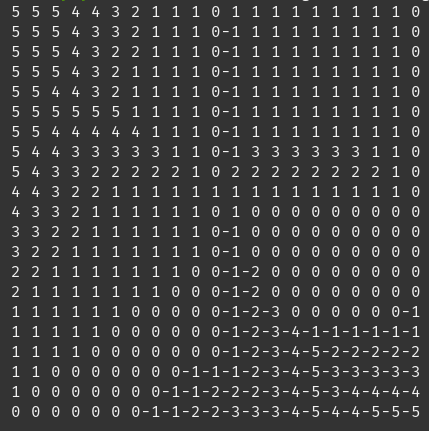
\includegraphics{printed_pi}
    \end{center}

\end{enumerate}
\end{document}
